\documentclass{article}
\usepackage{amsmath}
\usepackage{graphicx}

\begin{document}

\section{Lunar Regolith Properties}

%%%%%%%%%%%%%%%%%%%%%%%%%%%%%%%%%%%%%%%%%%%%%%%%%%%%%%%%%%%%%%%%%%%%%%
\subsection{Porosity}

The lunar regolith porosity is related to the amount of free space between individual grains. The greater the porosity, the more void space is present. Table 3.4.2.3.4-1 of the DSNE gives values of the porosity as a function of depth down to $60$ cm derived from Apollo core measurements (copied from Table 9.5 of the Lunar Sourcebook, \cite{heiken1991lunar}) and shown here in Table \ref{tab:porosity}.


\begin{table}[!htb]
	\begin{center}
		\caption{Porosity for various depths.}
		\label{tab:porosity}
		\begin{tabular}{c c}
			\hline
			Depth Range (cm)  & Average Porosity, n (\%)  \\
			\hline
			$0$ -- $15$  & $52\pm 2$  \\
			$0$ -- $30$  & $49\pm 2$   \\
			$30$ -- $60$ & $44\pm 2$   \\
			$0$ -- $60$  & $46\pm 2$  \\\hline
		\end{tabular}
	\end{center}
\end{table}


%%%%%%%%%%%%%%%%%%%%%%%%%%%%%%%%%%%%%%%%%%%%%%%%%%%%%%%%%%%%%%%%%%%%%%
\subsection{Density}

The bulk density ($\rho$) of the lunar regolith is defined as the mass of material in a given volume, which relates the particle density ($\rho_p$) and porosity ($n$) to the bulk density as (see Section 3.4.2.3.1 of the DSNE or Chapter 9 of the Lunar Sourcebook)
\begin{equation}
\rho = \rho_p(1-n).
\end{equation}

The DSNE suggests using $\rho_p = 3.1$ g/cm$^3$ for the average particle density over the entire Moon. Otherwise, the typical highlands particle density is $\rho_p = 2.75\pm 0.1$ g/cm$^3$ whereas the typical mare particle density is $\rho_p = 3.35\pm 0.1$ g/cm$^3$.

The bulk density\footnote{Follows the average particle density of $3.1$ g/cm$^3$ for all depths with a porosity depth dependence following Table \ref{tab:porosity}, see the \textit{porosity of lunar soil} paragraph on page 492 in the Lunar Sourcebook.} as a function of depth has been characterized multiple ways (Figure \ref{fig:regolith_density_vs_depth}). An empirical hyperbolic fit to in situ Apollo data takes the form
\begin{equation}\label{eq:regolith density vs depth}
\rho(z) = 1.92\frac{z+12.2}{z+18},
\end{equation}
where $z$ is the depth in cm and $\rho$ is in units of g/cm$^3$. Bulk density increases with depth. At the surface ($z=0$), the density is $1.30$ g/cm$^3$, and approaches $1.92$ g/cm$^3$ at the limits reached by the Apollo drill core samples, about $z=3$ m. In order to get an up-to-depth average of the bulk density, take
\begin{equation}
\rho_{avg, depth}(z) = \frac{1}{z}\int_{0}^{z}dz'\rho(z'), 
\end{equation}
which gives (compare with the equation for $d_m$ on page 494 of the Lunar Sourcebook)
\begin{equation}\label{eq:density depth averaged}
\rho_{avg, depth}(z) = 1.92\left[1 - \frac{5.8\ln\left(\frac{z + 18}{18}\right)}{z}\right].
\end{equation}
For example, the average bulk density of the regolith with a depth range of $0$ -- $60$ cm would be $\rho_{avg, depth}(60)$ = $1.65$ g/cm$^3$.



\begin{figure}[!htb]
	\centering
	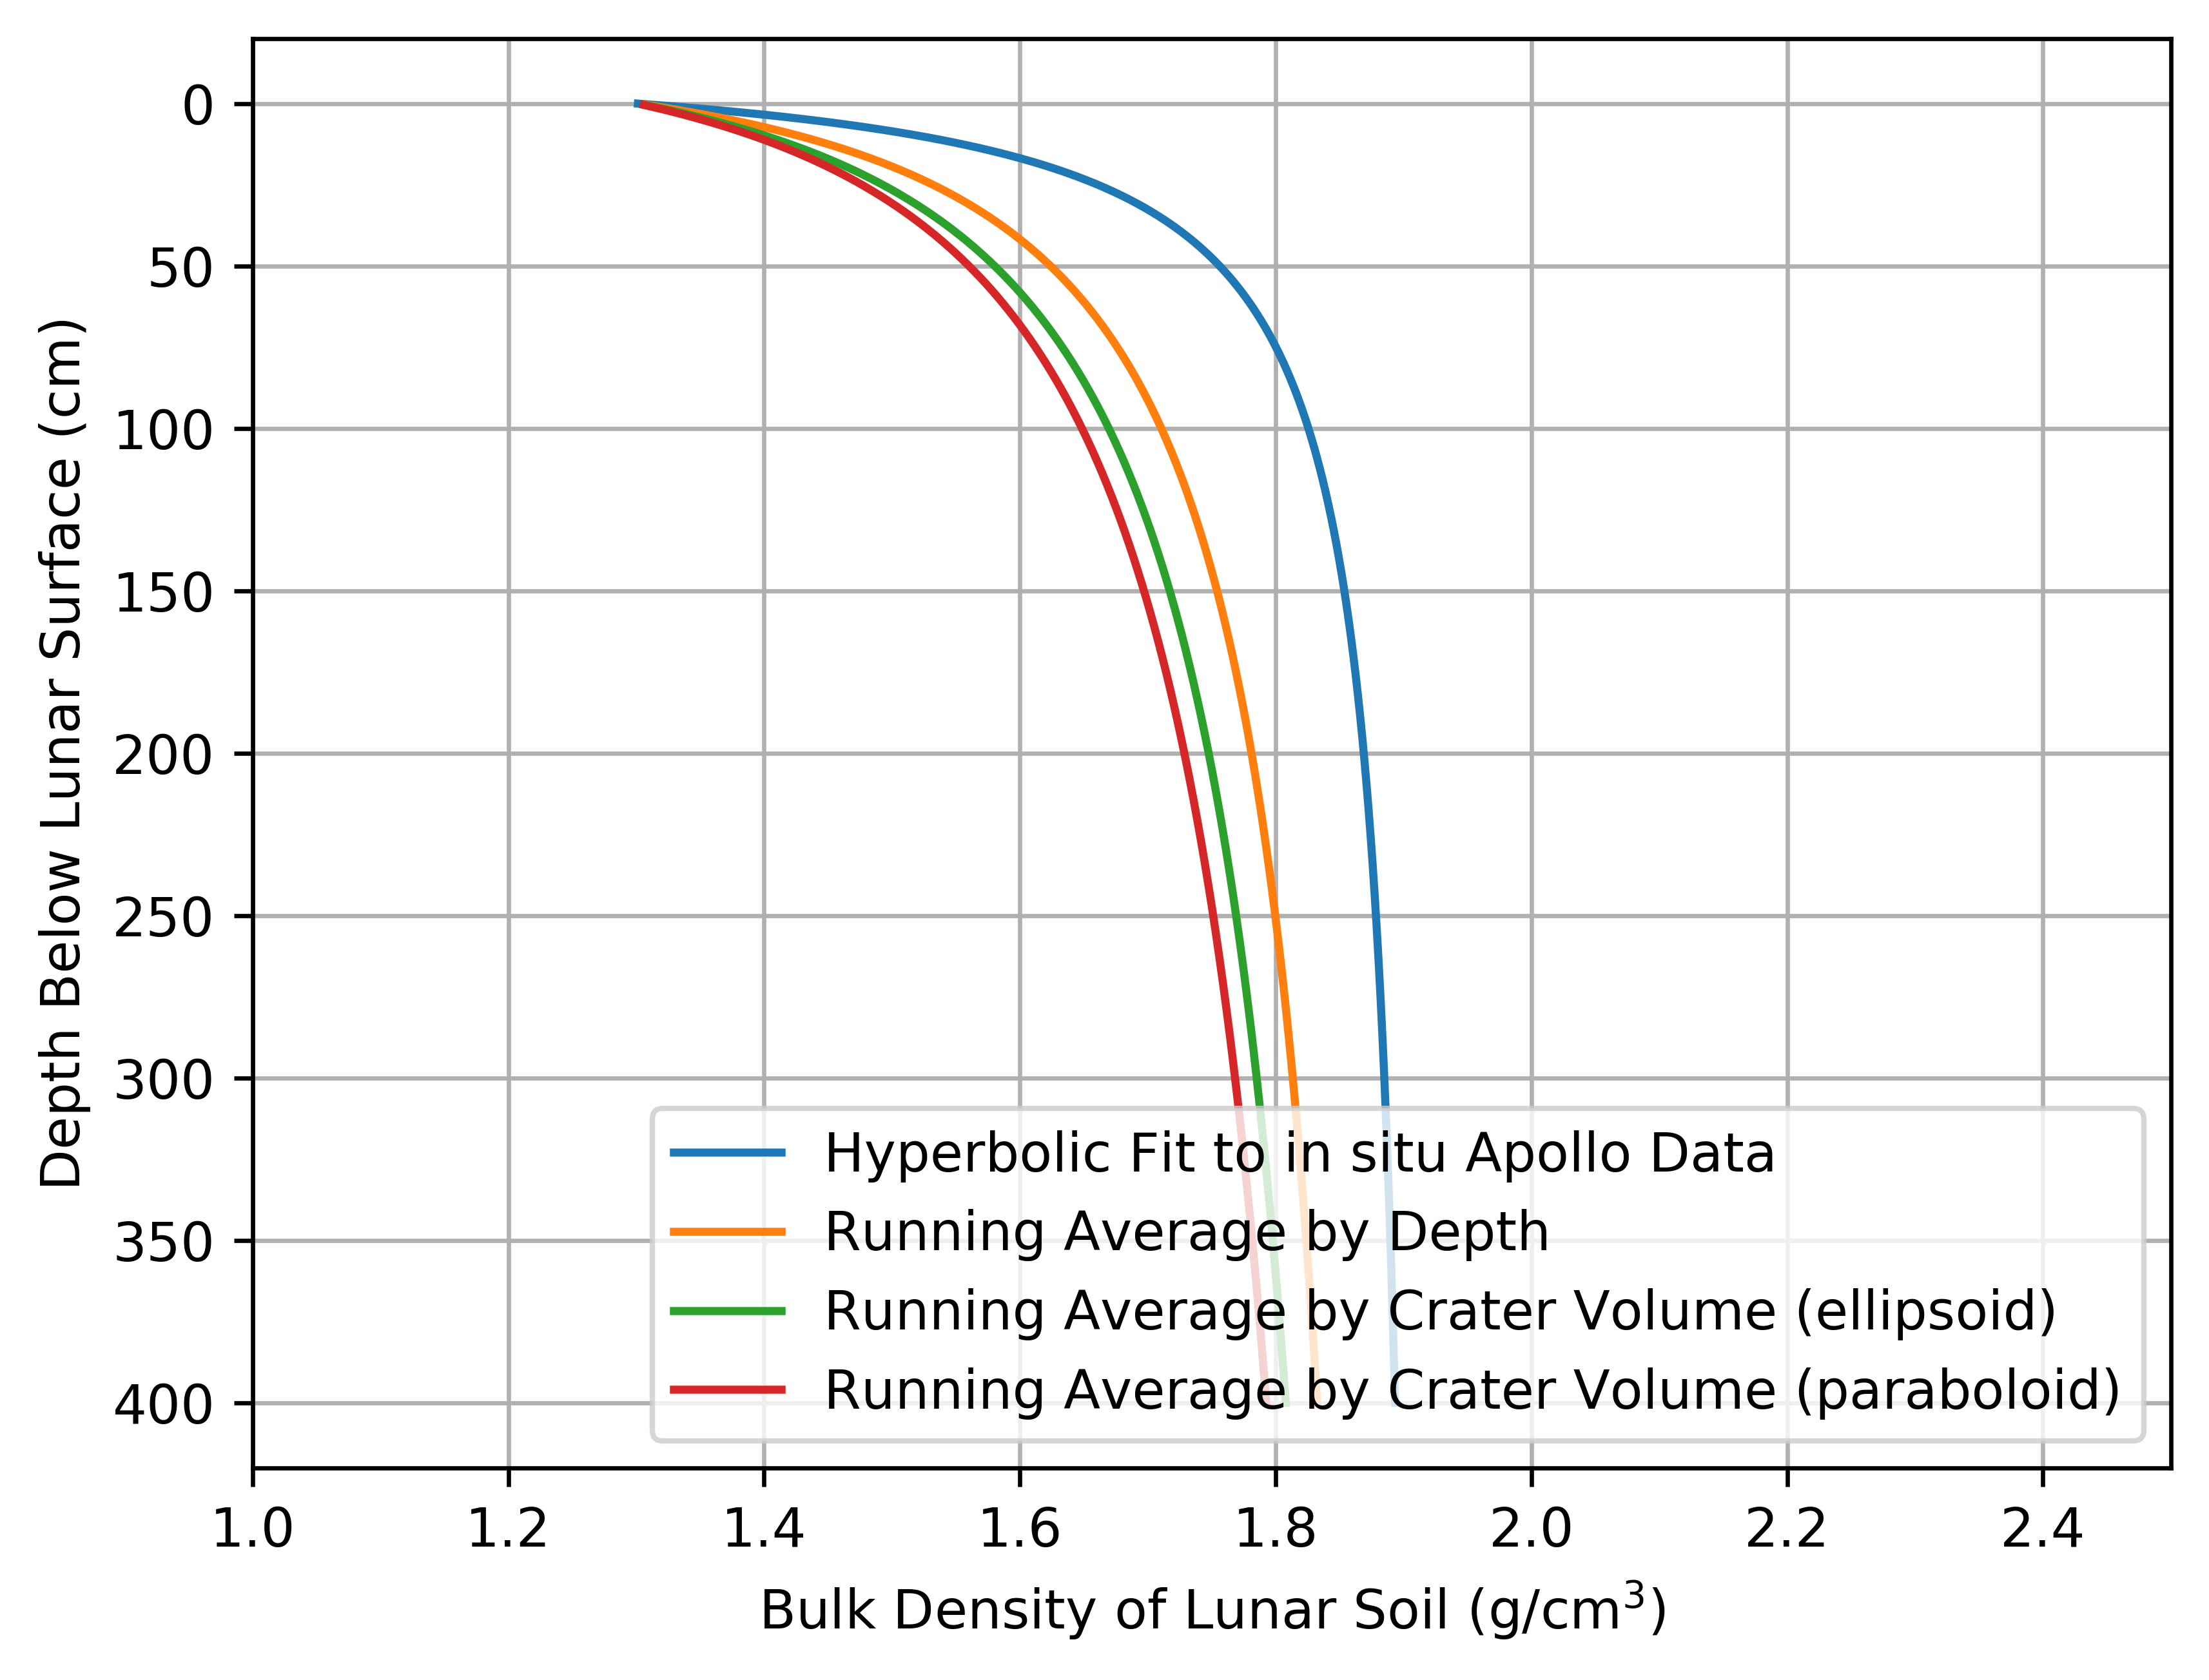
\includegraphics[width=\linewidth]{regolith_density_vs_depth.png}
	\caption{A comparison of the regolith bulk density for a certain depth depth (blue), the depth-averaged bulk density (orange), and the volume-averaged bulk density (green). See also, Figure 9.16 of the Lunar Sourcebook \citep{heiken1991lunar}.}
	\label{fig:regolith_density_vs_depth}
\end{figure}

For a higher-fidelity estimate of the average bulk density sampled by an impact crater, a volume-average can be used instead of a depth-average, given by
\begin{equation}\label{eq:density volume averaged def}
\rho_{avg, volume}(z) = \frac{\int dV \rho(z')}{\int dV}.
\end{equation}
Expanding the integral in a cylindrical coordinate system and assuming an ellipsoidal crater shape, Equation \eqref{eq:density volume averaged def} becomes
\begin{align}
\rho&_{avg, ellipsoid}(z) = \frac{\int_{0}^{z}\int_{0}^{R\sqrt{1-z'^2/z^2}}\int_{0}^{2\pi}d\phi rdr dz' \rho(z')}{\int_{0}^{z}\int_{0}^{R\sqrt{1-z'^2/z^2}}\int_{0}^{2\pi}d\phi rdr dz'}\\\label{eq:density volume averaged}
&= \frac{1.92}{4z^3}\left[z(6ab - 6b^2 - 3az + 3bz + 4z^2) + 6(a-b)(b^2-z^2)\ln\left(\frac{b}{z + b}\right)\right],
\end{align}
for the volume-averaged density in g/cm$^3$ with $z$ in cm, where $a = 12.2$ and $b = 18$. Comparing to the earlier example, the average bulk density of the regolith with a depth range of $0$ -- $60$ cm would be $\rho_{avg, ellipsoid}(60)$ = $1.60$ g/cm$^3$; $\sim 3\%$ less than $\rho_{avg, depth}(60) = 1.65$ g/cm$^3$.

Instead of an ellipsoidal shape, if a paraboloid crater shape is assumed, Equation \eqref{eq:density volume averaged def} becomes
\begin{align}
\rho_{avg, paraboloid}(z) &= \frac{\int_{0}^{z}\int_{0}^{R\sqrt{1-z'/z}}\int_{0}^{2\pi}d\phi rdr dz' \rho(z')}{\int_{0}^{z}\int_{0}^{R\sqrt{1-z'/z}}\int_{0}^{2\pi}d\phi rdr dz'}\\\label{eq:density volume averaged_para}
&= \frac{1.92}{z/2}\left[b-a + \frac{z}{2} - \frac{(a-b)(b+z)\ln\left(\frac{b}{z+b}\right)}{z}\right],
\end{align}
using the same values for $a$ and $b$ as before. Again, comparing to the prior depth average example, the average bulk density of the regolith with a depth range of $0$ -- $60$ cm would be $\rho_{avg, paraboloid}(60)$ = $1.58$ g/cm$^3$; $\sim 4\%$ less than $\rho_{avg, depth}(60) = 1.65$ g/cm$^3$. The expression given in Equation \eqref{eq:density volume averaged_para} is useful for computing the ejected mass from a crater\footnote{In an iterative fashion, since the crater radius depends on the regolith density.}, given a crater depth $z$.





The expressions for the regolith density at a certain depth $z$, weighted by depth, and weighted by crater volume (ellipsoid and paraboloid) are given by Equations \eqref{eq:regolith density vs depth}, \eqref{eq:density depth averaged}, and \eqref{eq:density volume averaged}, \eqref{eq:density volume averaged_para}, respectively (Figure \ref{fig:regolith_density_vs_depth}). The relative error between the different methods are shown in Figure \ref{fig:ratio_of_avg_bulk_density}. The crater volume is approximated as a half-ellipsoid with two of the dimensions scaled by the crater radius $R$ and one dimension scaled by the crater depth $z$, sliced such that the half-ellipsoid is symmetric about the surface normal for Equation \eqref{eq:density volume averaged}. On the other hand, a paraboloid-shaped crater is used for Equation \eqref{eq:density volume averaged_para}. For a given crater, more of the volume is near the surface so that more weight is given by bulk densities that originate near the surface. In contrast, the depth-averaged bulk density takes the bulk density at each depth equally. This results in the volume-averaged bulk density to be slightly less than the depth-averaged bulk density, as shown in Figure \ref{fig:regolith_density_vs_depth}. In addition, comparing an ellipsoidal crater vs.\ a parabolic crater, the parabolic crater (typically used in literature, see \cite{singer2020lunar}) exhibits the softest increase of the average bulk density as a function of depth.

The lunar meteoroid ejecta model currently uses a constant regolith density for all depths for simplicity. The higher fidelity expressions shown above are for future reference if it is found that the regolith density has an important effect on the final environment.


\begin{figure}[!htb]
	\centering
	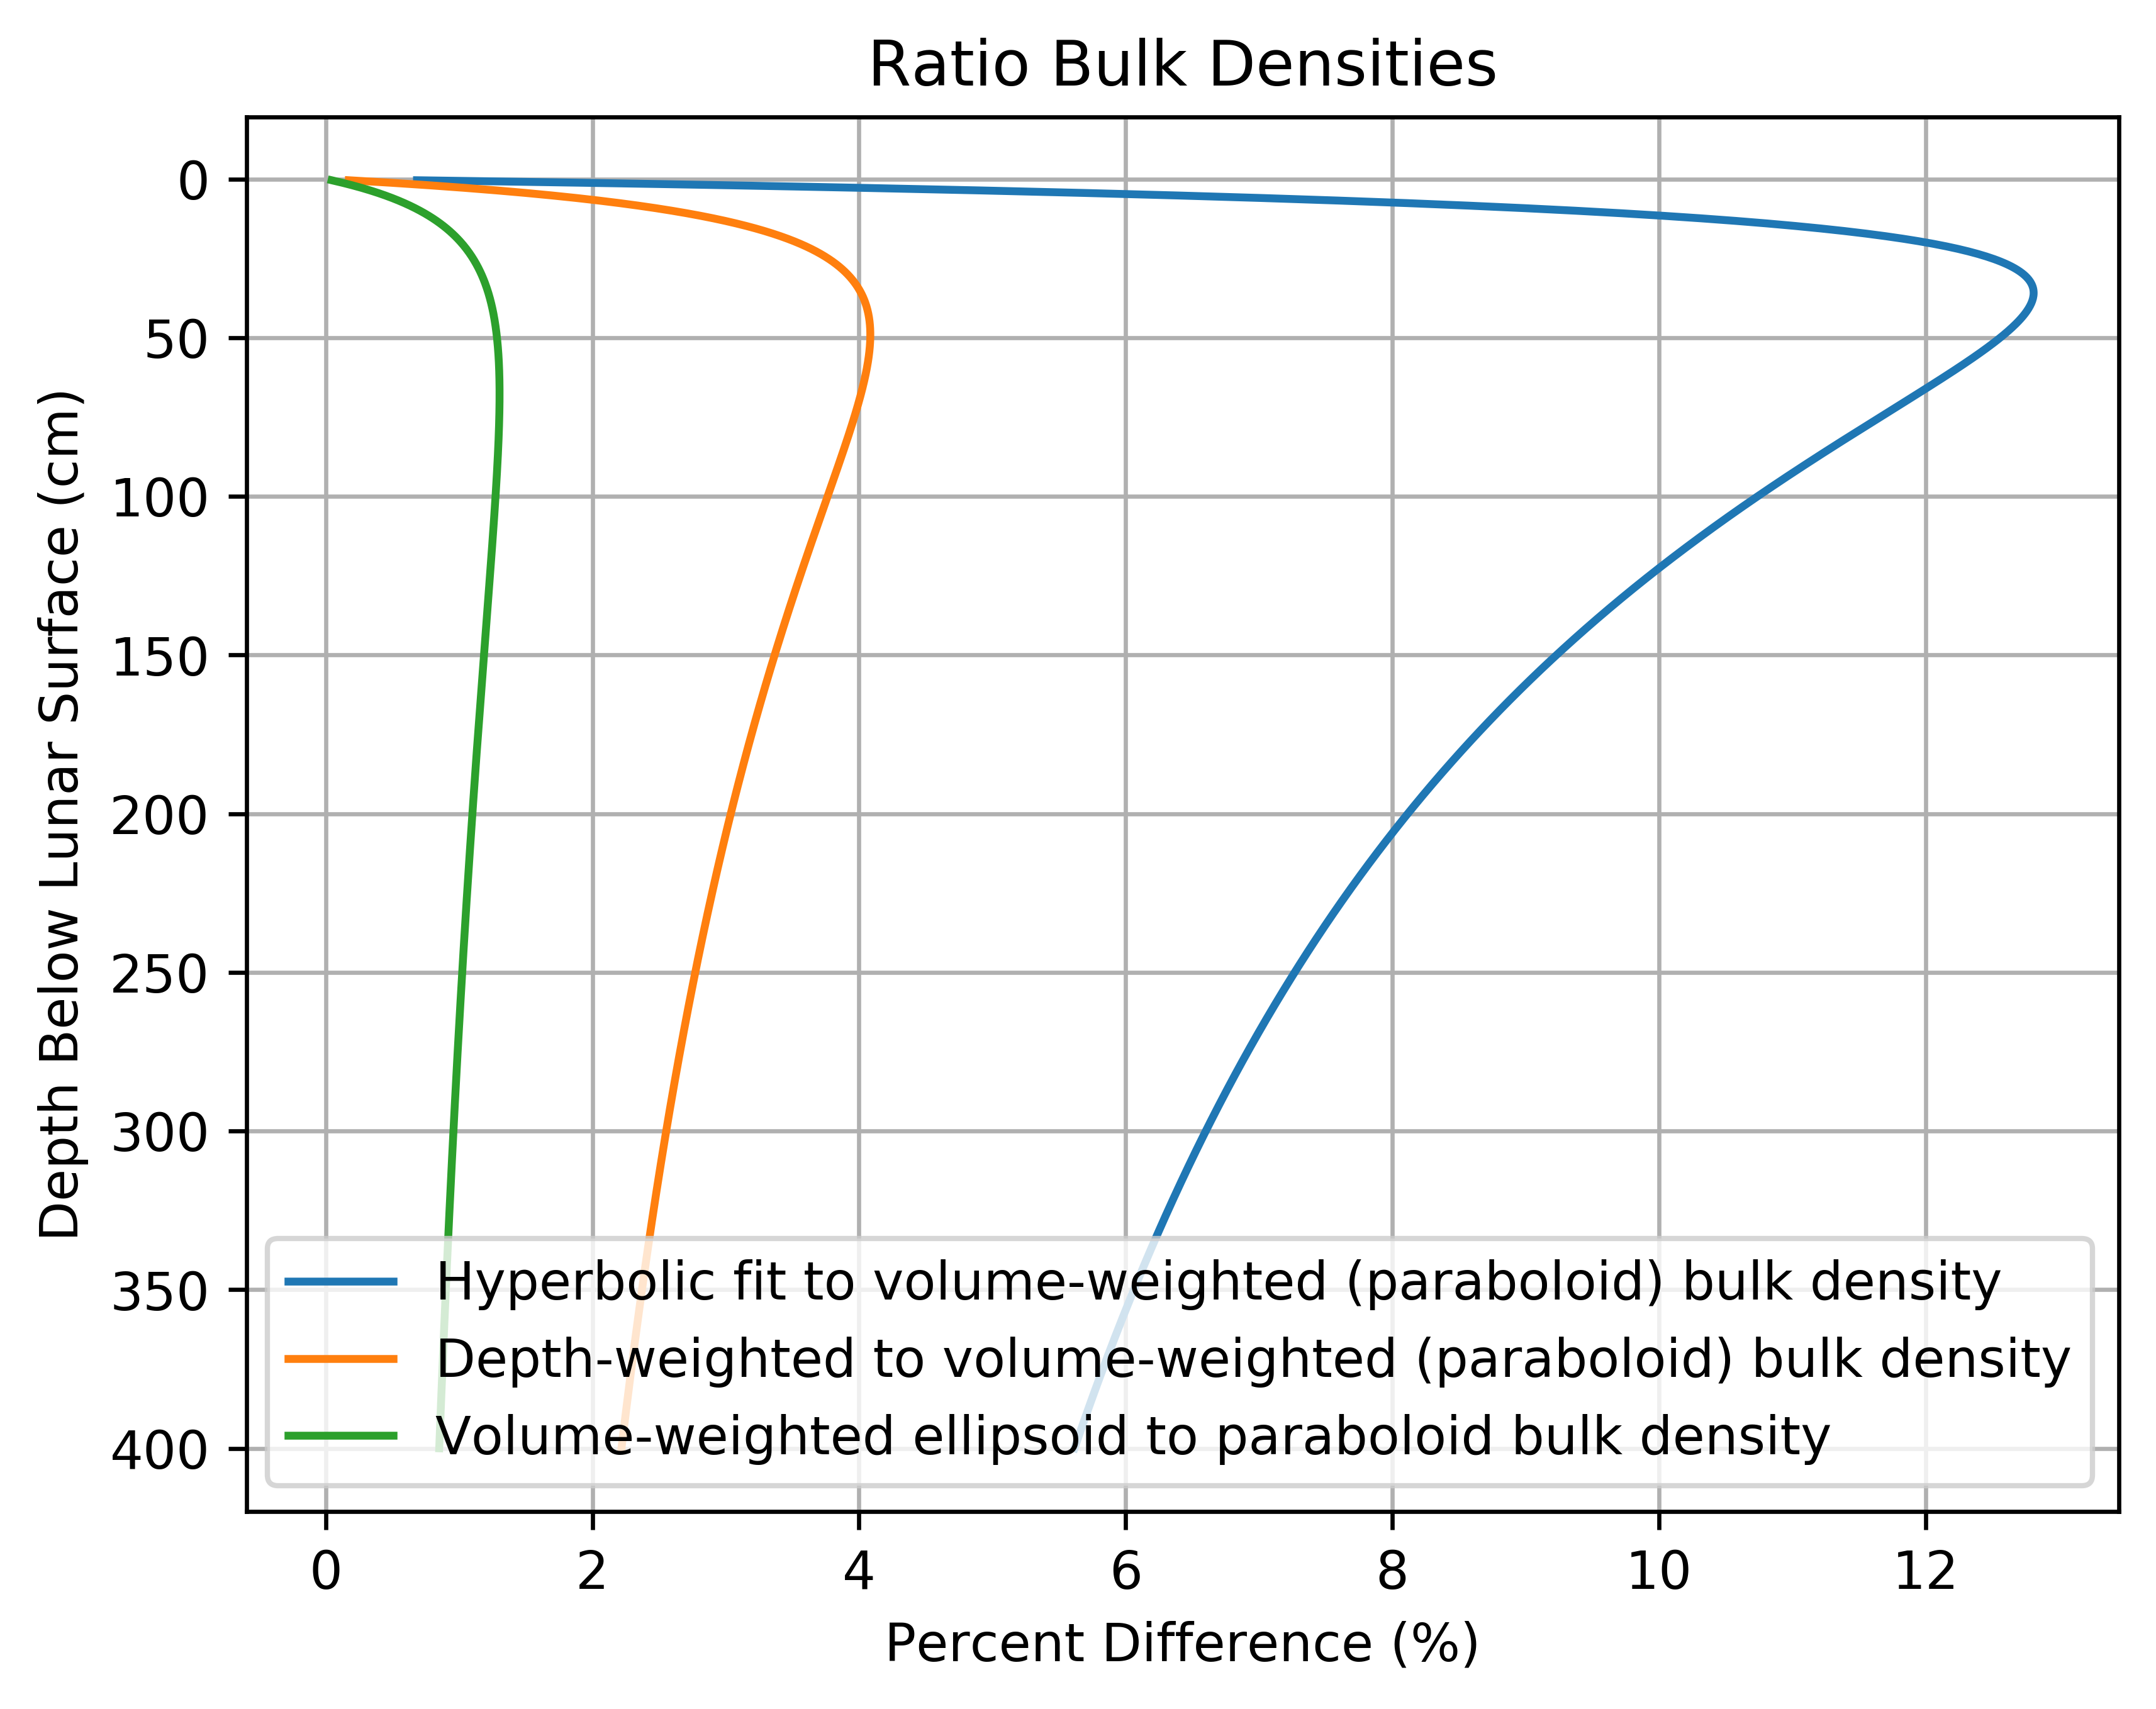
\includegraphics[width=\linewidth]{ratio_of_avg_bulk_density.png}
	\caption{Relative error of using the density at a certain depth (blue) and using the depth-weighted average (orange) of the regolith bulk density.}
	\label{fig:ratio_of_avg_bulk_density}
\end{figure}


%%%%%%%%%%%%%%%%%%%%%%%%%%%%%%%%%%%%%%%%%%%%%%%%%%%%%%%%%%%%%%%%%%%%%%
\subsection{Strength}

The regolith includes fine-grained material from the lunar surface down to $\sim10$ m depth. The large-scale, coarse grained ejecta that is ballistically transported resides from $10$ m to about $2$ km below the surface (Fig 4.22 of the Lunar Sourcebook, \cite{heiken1991lunar}). 

The strength of the regolith can be measured in different ways, depending on the use. In the case of modeling impacts, the shear strength \citep[see Section 3 of][]{housen2011ejecta} of loose regolith and tensile strength of solid rock can be used. Since all of the impacts studied in this model will create craters less than $2$ km, the shear strength was used for both loose regolith and large scale ejecta material. The shear strength of the lunar soil increases with depth, as depicted by both Figure 9.26 of the Lunar Sourcebook (reproduced in Figure \ref{fig:shear_strength_vs_depth}) and Table 12 of \cite{slyuta2014physical}, shown in Table \ref{tab:shear_strength}.

\begin{table}[!htb]
	\begin{center}
		\caption{The change of the shear strength of the lunar soil with depth.}
		\label{tab:shear_strength}
		\begin{tabular}{c c}
			\hline
			Depth (cm)  & Shear strength (kPa)  \\
			\hline
			$5$  & $0.1$ -- $2.5$  \\
			$50$  & $1$ -- $3.5$   \\
			$100$ & $2$ -- $4$  \\
			$200$  & $4$ -- $8$  \\\hline
		\end{tabular}
	\end{center}
\end{table}

\begin{figure}[!htb]
	\centering
	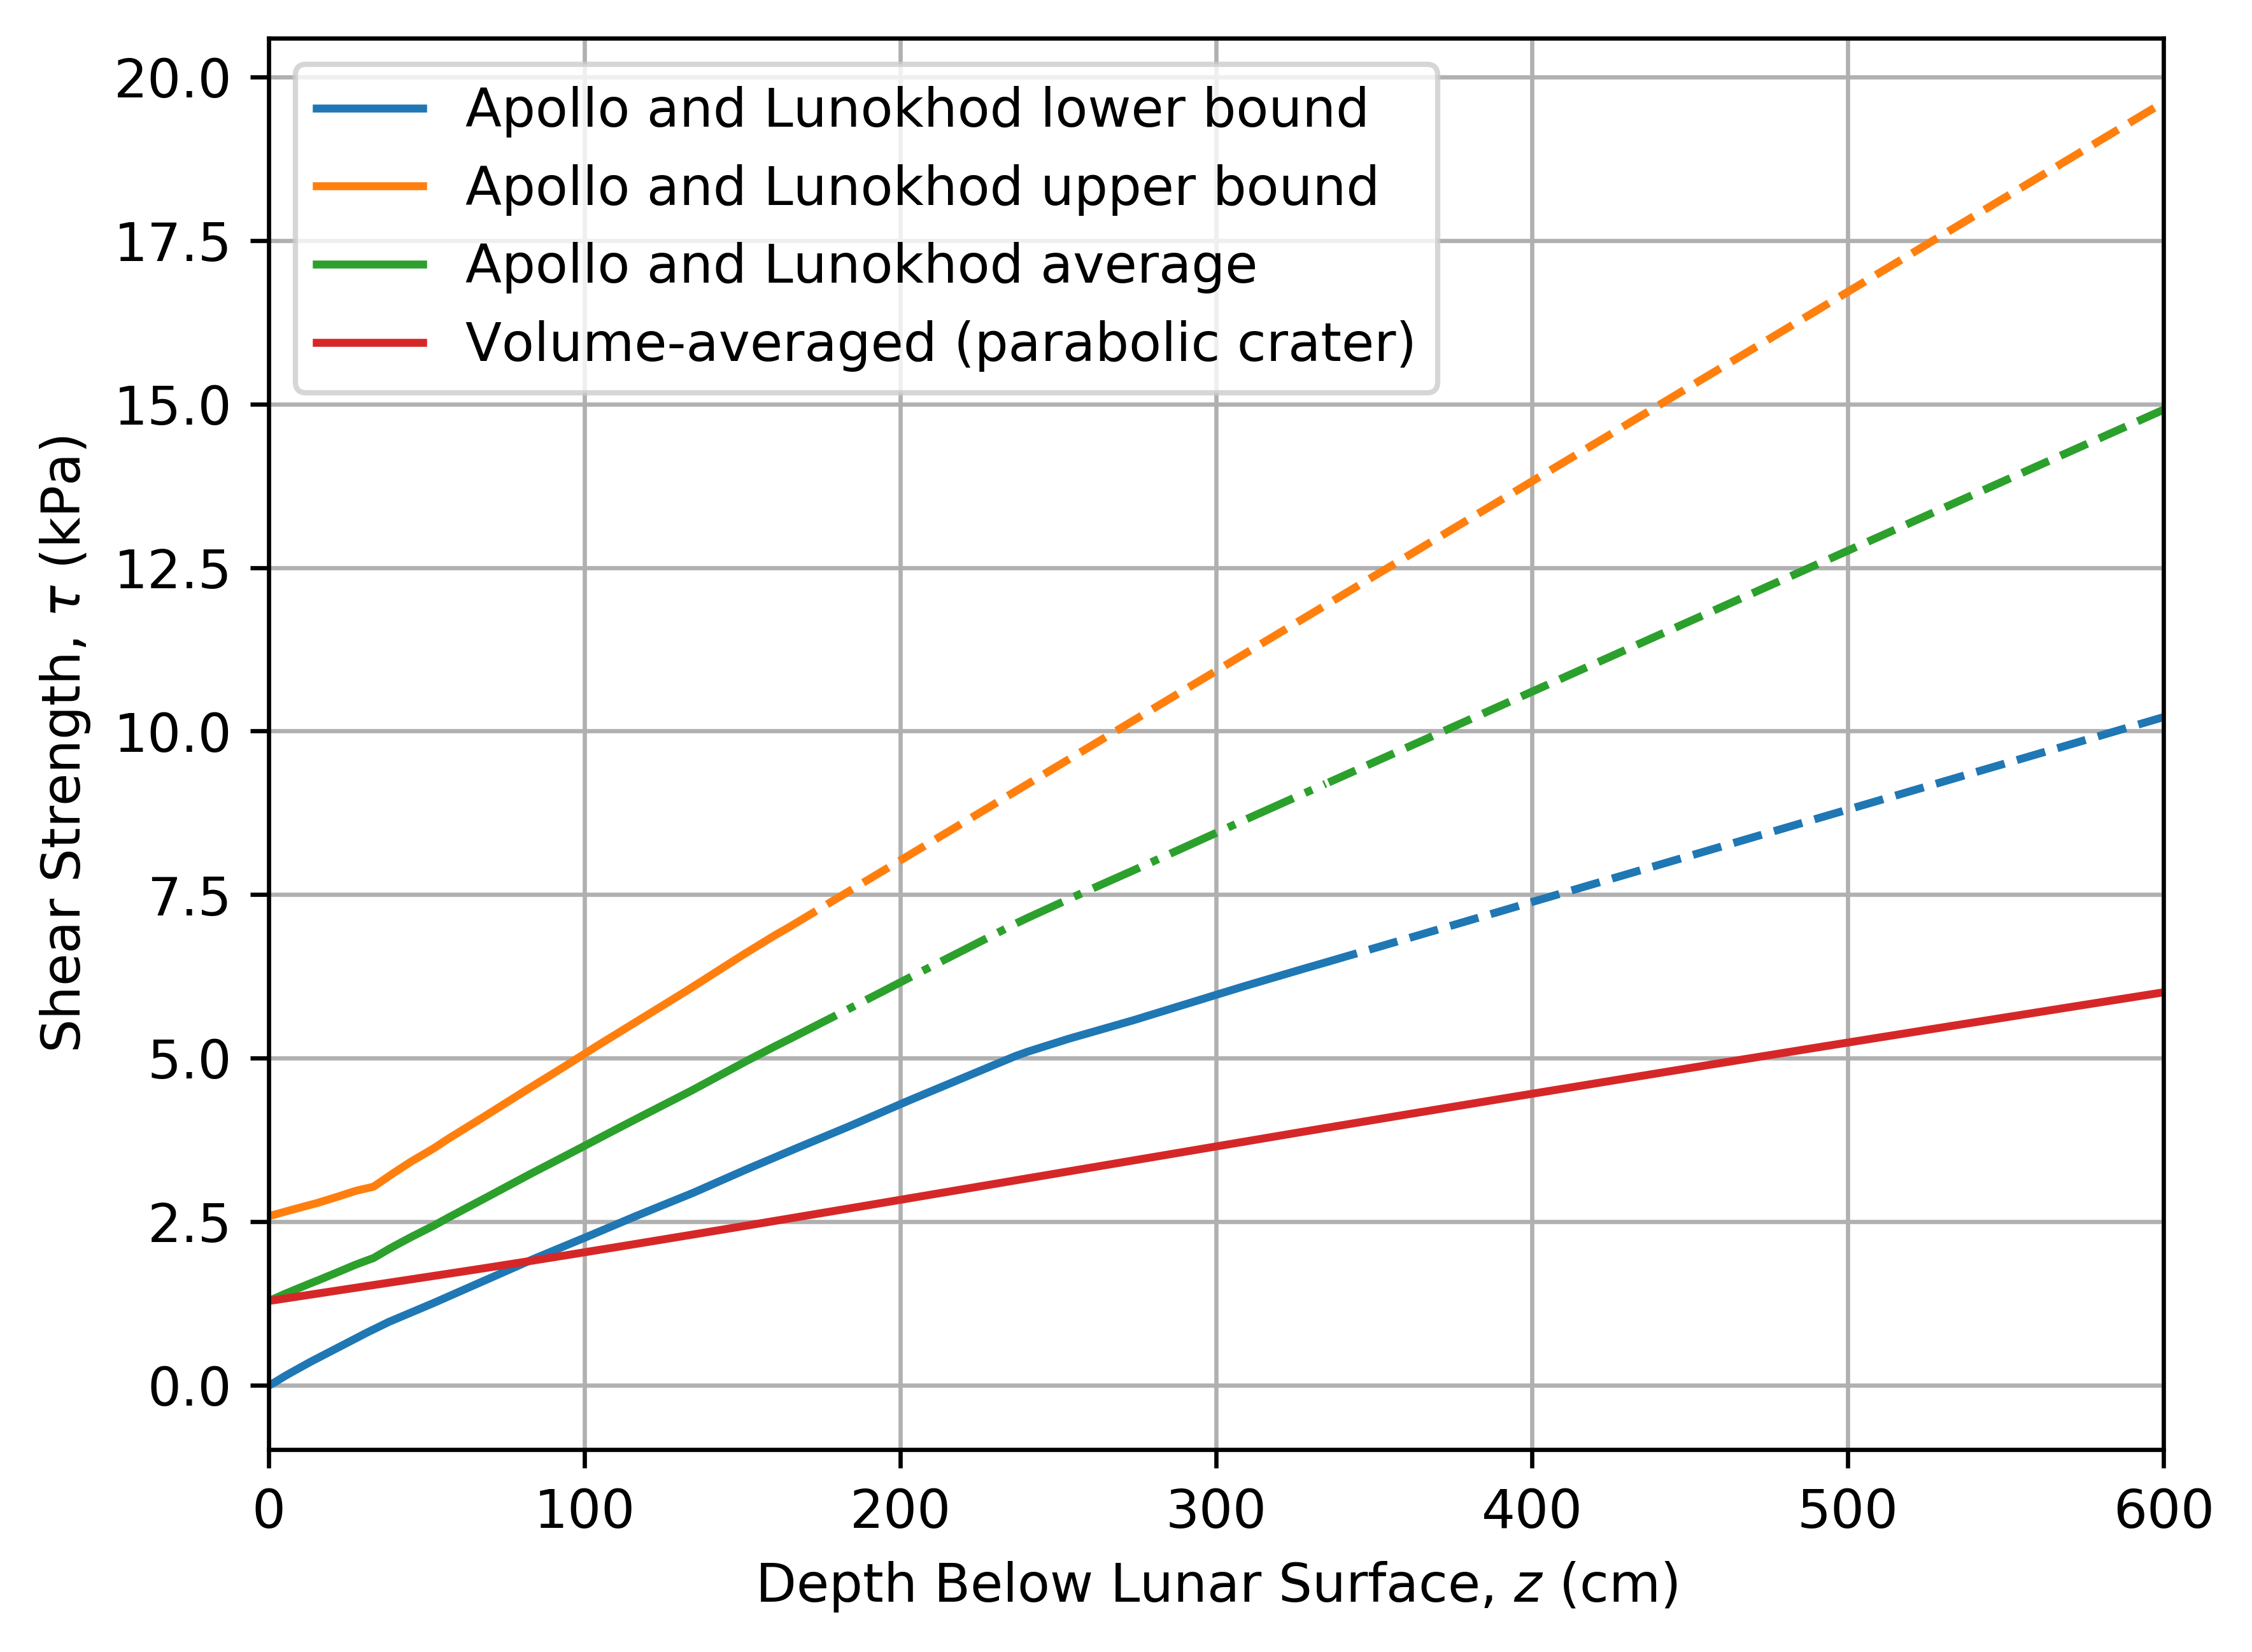
\includegraphics[width=\linewidth]{shear_strength_vs_depth.png}
	\caption{The range of regolith shear strength as a function of depth below the lunar surface taken from Figure 9.26 of the Lunar Sourcebook. The average shear strength is also calculated (green). Dashed lines indicate extrapolated points beyond available data. The volume-averaged shear strength (red) assumes a parabolic-shaped crater of depth $z$.}
	\label{fig:shear_strength_vs_depth}
\end{figure}

The average shear strength (green curve) in Figure \ref{fig:shear_strength_vs_depth} can be expressed by the piece-wise form
\begin{equation}\label{eq:shear strength}
\tau(z) =
\begin{cases}
\frac{z}{45.55} + 1.288,\text{   $0 \le z < 50$ cm}\\
\frac{z}{40.21} + 1.144,\text{   $50$ cm $\le z < 250$ cm}\\
\frac{z}{46.06} + 1.942,\text{   $z \ge 250$ cm}
\end{cases}.
\end{equation}
Assuming the crater has a parabolic shape and that the effective shear strength is the volume-average (similar approach to Equation \eqref{eq:density volume averaged def}), Equation \eqref{eq:shear strength} becomes
\begin{equation}\label{eq:shear strength_avg_para}
\tau(z) =
\begin{cases}
\frac{z}{136.65} + 1.288,\text{   $0 \le z < 50$ cm}\\
\frac{z}{120.63} + 1.144 + \frac{7.163}{z} - \frac{118.33}{z^2},\text{   $50$ cm $\le z < 250$ cm}\\
\frac{z}{138.18} + 1.942 - \frac{194.81}{z} + \frac{16902}{z^2},\text{   $z \ge 250$ cm}
\end{cases},
\end{equation}
as shown by the red curve in Figure \ref{fig:shear_strength_vs_depth}.



%%%%%%%%%%%%%%%%%%%%%%%%%%%%%%%%%%%%%%%%%%%%%%%%%%%%%%%%%%%%%%%%%%%%%%
\subsection{Particle Size Distribution}

The cumulative distribution function (CDF) of the regolith particle sizes\footnote{In the context here, particle size is defined as the particle diameter of a spherical-shaped particle. Other sections may define size by the radius.} are fit to several Apollo samples, as shown in Figure~\ref{fig:Carrier2003_Fig1_particle-size-distribution}. An impact may modify and reorganize preexisting particle size distributions depending on the ejected speed (see Section \ref{ssec:Mass/Particle Size Distribution}). For this section, however, the unmodified regolith size distribution is given for reference.
\begin{figure}[h!]
	\centering
	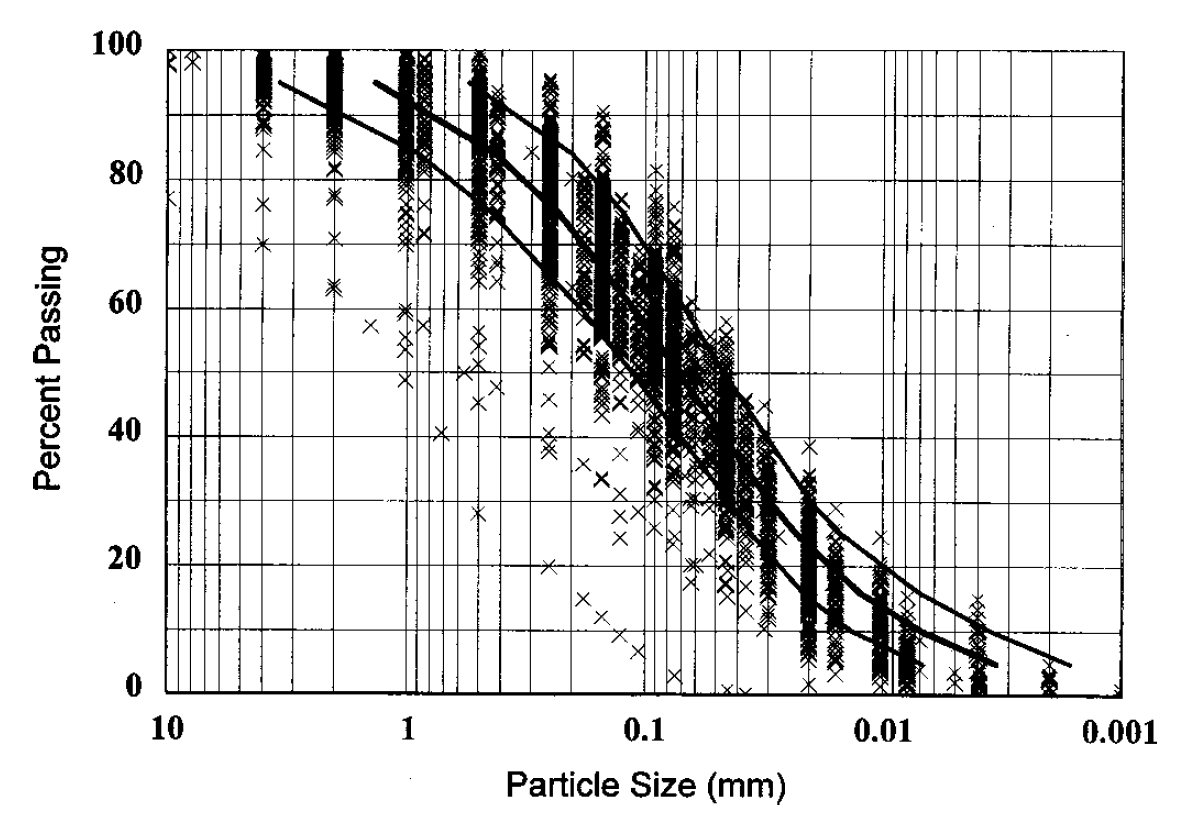
\includegraphics[scale=0.4]{Carrier2003_Fig1_particle-size-distribution.PNG}
	\caption{Geotechnical particle size distribution: middle curve showing the average distribution; left-hand and right-hand curves showing $\pm$1 standard deviation \citep{carrier2003particle}. Note, that the percent passing is normalized by mass and not particle number \citep[see][]{carrier1973lunar}.}\label{fig:Carrier2003_Fig1_particle-size-distribution}
\end{figure}
The digitized data from Figure \ref{fig:Carrier2003_Fig1_particle-size-distribution} is shown in Table \ref{tab:Carrier2003}.
\begin{table}
	\centering
	\caption{Digitized data points from Figure \ref{fig:Carrier2003_Fig1_particle-size-distribution}, see \cite{carrier2003particle}.}\label{tab:Carrier2003}
	\csvautotabular{Carrier2003_digitized.csv}
\end{table}


\begin{figure}[h!]
	\centering
	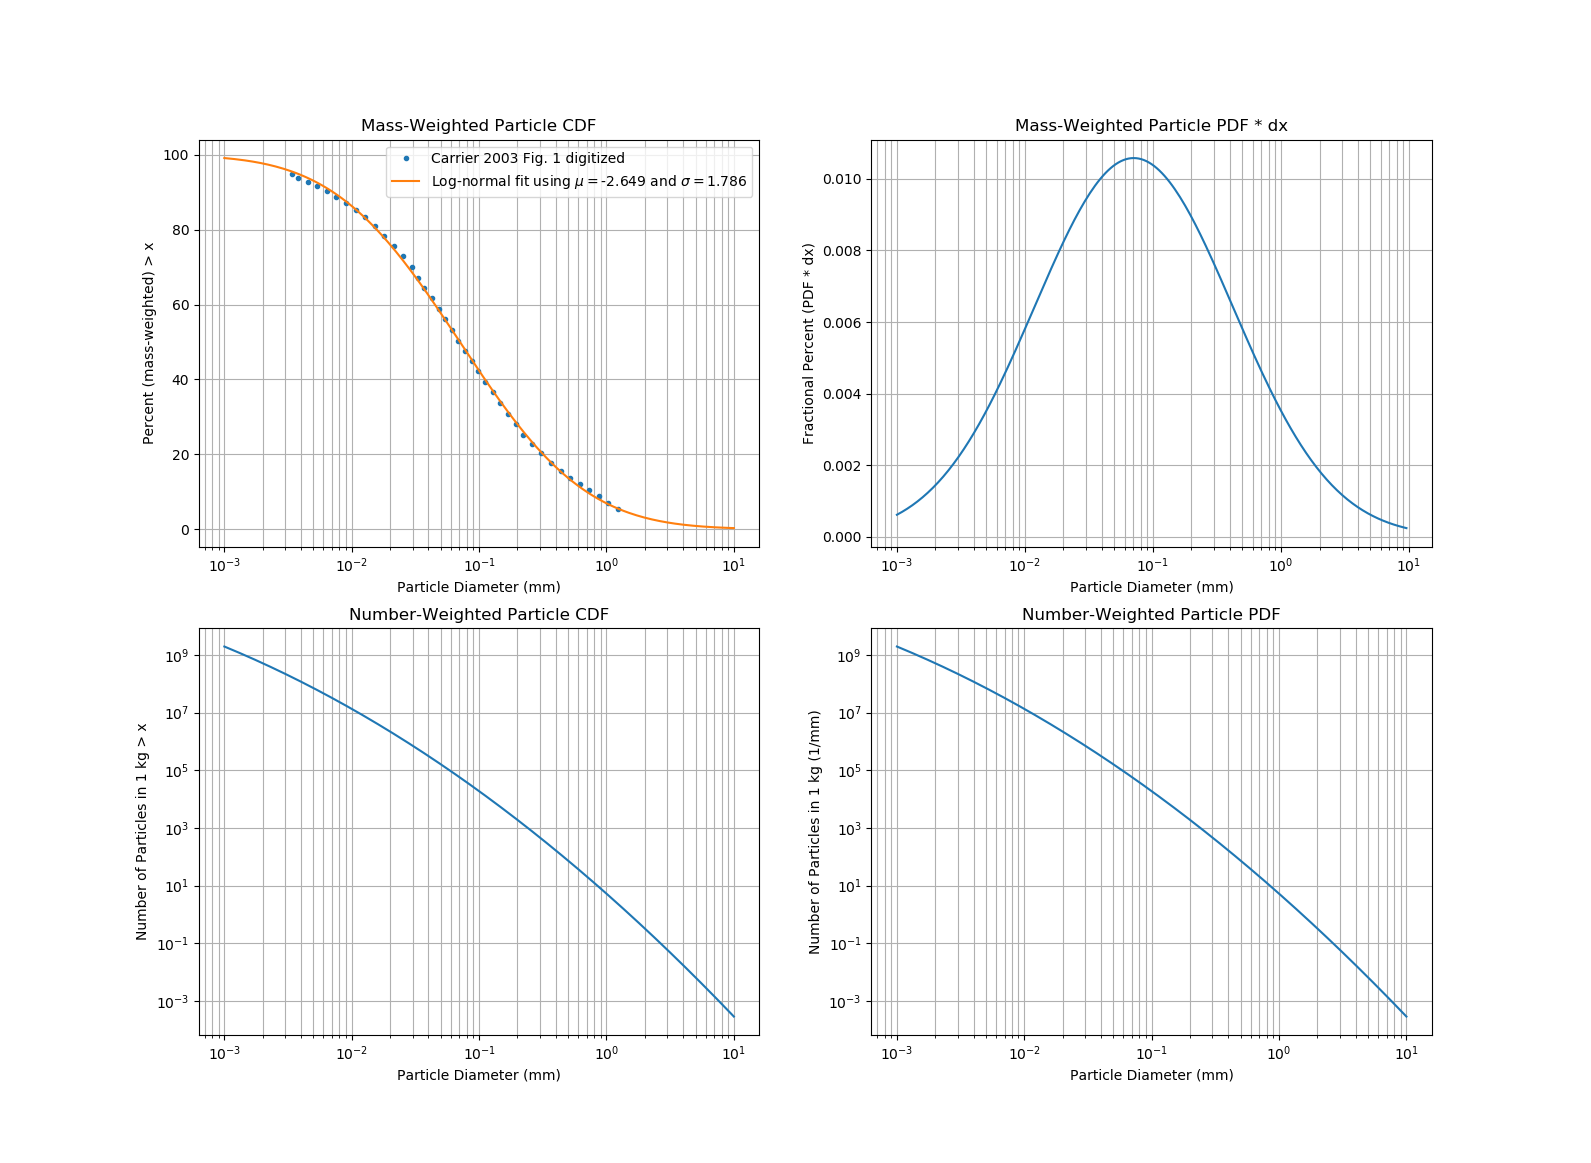
\includegraphics[width=1.1\textwidth]{Carrier2003_CDFs_PDFs.png}
	\caption{Plots of the mass-weighted and number-weighted CDFs and PDFs derived from \cite{carrier2003particle}. Top left: the digitized data from Figure 1 of \cite{carrier2003particle} is shown with the log-normal distribution fit. Top right: The mass-weighted PDF * dx is shown to indicate what particle size dominates the contribution of mass. Bottom left: The number-weighted CDF showing number of particles in 1 kg of regolith greater than a size $x$. Bottom right: The number-weighted PDF is shown in units of mm$^{-1}$.}\label{fig:Carrier2003_CDFs_PDFs}
\end{figure}

\cite{carrier2003particle} specifically called out that the mass-weighted CDF can be modeled by a log-normal distribution. This assumption is made below. By definition, a log-normal distribution is given by
\begin{equation}
F_{\text{kg}}(>x) = 1 - F_{\text{kg}}(<x) = \frac{1}{2}\left[1 - \text{erf}\left(\frac{\ln x - \mu}{\sqrt{2}\sigma}\right)\right],
\end{equation}
where $x$ is the particle diameter size in units of mm, $\mu$ is the expected value of $\ln x$, and $\sigma$ is the standard deviation of $\ln x$.

The PDF is then given by
\begin{equation}
f_{\text{kg}}(x) = \frac{1}{\sigma\sqrt{2\pi}}\frac{1}{x}\exp\left[-\frac{(\ln x - \mu)^2}{2\sigma^2}\right].
\end{equation}

In order to have the number-weighted PDF and CDF, we begin with $f_{\text{kg}}(x)$ and divide by the mass of a given particle size (diameter), \citep[e.g., Equation (7) of~][]{koschny2001impacts_mass}
\begin{equation}
m(x) = \frac{\pi}{6}\rho x^3,
\end{equation}
so that we have (assuming $F_{\text{kg}}$ represents the CDF for 1 kg of regolith)
\begin{equation}
f_{\text{number}}(x) = \frac{f_{\text{kg}}(x)}{m(x)} = \frac{6}{\pi\rho}\frac{1 \text{kg}}{1 \text{mm}^3}\frac{1}{\sigma\sqrt{2\pi}}
\frac{1}{x^4}\exp\left[-\frac{(\ln x - \mu)^2}{2\sigma^2}\right],
\end{equation}
for the number-weighted PDF. To arrive at the number-weighted CFD, integration over $f_{\text{number}}(x)$ is done such that
\begin{equation}
F_{\text{number}}(>x) = \int_{x}^{\infty}dx' f_{\text{number}}(x').
\end{equation}
Solving the integral, the number-weighted CDF is given by
\begin{equation}\label{eq:number_CFD_regolith}
F_{\text{number}}(>x) = \frac{6}{\pi\rho}\frac{1 \text{kg}}{1 \text{mm}^3}\frac{1}{\sigma\sqrt{2\pi}}
\left[1 - \text{erf}\left(\frac{\ln x - \mu + 3\sigma^2}{\sqrt{2}\sigma}\right)\right]\exp\left(-3\mu + \frac{9\sigma^2}{2}\right),
\end{equation}
which is the number of particles of diameter $x$ or greater in 1 kg of regolith. For $F_{\text{number}}(<x)$, flip the minus sign to a plus sign on the error function\footnote{Note that $\text{erfc}(x) = 1- \text{erf}(x)$.}.

Fitting the mass-weighted CDF $F(<x)$ to Figure \ref{fig:Carrier2003_Fig1_particle-size-distribution}, the following parameters are obtained:
\begin{align}
\mu &= -2.649,\\
\sigma &= 1.786,
\end{align}
where the mean, median, and mode particle size (weighted by mass) is
\begin{align}
x_{\text{mean}} &= \exp\left(\mu + \frac{\sigma^2}{2}\right) = 34.8 \text{$\mu$m},\\
x_{\text{median}} &= \exp(\mu) = 7.07 \text{$\mu$m},\\
x_{\text{mode}} &=  \exp\left(\mu - \sigma^2\right) = 0.291 \text{$\mu$m}.
\end{align}

If the mean, median, and mode particle size weighted by number are needed, then the modified parameters are
\begin{align}
\mu^\star &= \mu - 3\sigma^2 = -12.22,\\
\sigma^\star &= \sigma = 1.786,
\end{align}
giving the following (now weighted by number):
\begin{align}
x^\star_{\text{mean}} &= \exp\left(\mu^\star + \frac{\sigma^{\star 2}}{2}\right) = 2.43 \text{ nm},\\
x^\star_{\text{median}} &= \exp(\mu^\star) = 0.494 \text{ nm},\\
x^\star_{\text{mode}} &=  \exp\left(\mu^\star - \sigma^{\star 2}\right) = 0.0203 \text{ nm}.
\end{align}
Note that these set of averages are outside the range of the data provided in \cite{carrier2003particle} and are only valid if the log-normal distribution holds for these very small particles. This regime is on the order of several atomic nuclei large.


As an example, if the number of particles greater than 1 $\mu$g per 1 kg of regolith are needed, then use Equation \eqref{eq:number_CFD_regolith} (assuming a regolith density of $\rho$ = 3.1 g / cm$^3$ such that $x(1 \mu\text{g}) = 8.509 \mu\text{m}$)
\begin{equation}
F_{\text{number}}(> x = 8.509 \mu\text{m}) = 3.146\times 10^{7} \text{ \# of particles per 1 kg of regolith}.
\end{equation}






\end{document}